\documentclass[acmtog]{acmart}
\usepackage{graphicx}
\usepackage{subfigure}
\usepackage{natbib}
\usepackage{listings}
\usepackage{bm}

\definecolor{blve}{rgb}{0.3372549 , 0.61176471, 0.83921569}
\definecolor{gr33n}{rgb}{0.29019608, 0.7372549, 0.64705882}
\makeatletter
\lst@InstallKeywords k{class}{classstyle}\slshape{classstyle}{}ld
\makeatother
\lstset{language=C++,
	basicstyle=\ttfamily,
	keywordstyle=\color{blve}\ttfamily,
	stringstyle=\color{red}\ttfamily,
	commentstyle=\color{magenta}\ttfamily,
	morecomment=[l][\color{magenta}]{\#},
	classstyle = \bfseries\color{gr33n}, 
	tabsize=2
}
\lstset{basicstyle=\ttfamily}

% Title portion
\title{Assignment1:\\ {Exploring OpenGL Programming}} 

\author{Name:\quad Yang Hongdi \\ student number:\ 2019533234
\\email:\quad yanghd@shanghaitech.edu.cn}

% Document starts
\begin{document}
\maketitle

\vspace*{2 ex}

\section{Introduction}
\quad The program is able to load vertex data from file. The scene contains one direction light and 3 point lights. You can change the model by pressing "X" on keyboard.
You can also move and rotate the camera by using mouse and keyboard.
\section{Implementation Details}
\subsection{Loading data}
\quad For Data Loading, I did it in mesh.cpp and use filestream and stringstream to load the data line by line.
Here are some of the codes.\\
	\begin{lstlisting}
  std::ifstream fin(path.c_str());
  std::vector<std::string> lines;
  std::string readline;
  getline(fin, readline);
  std::stringstream ss(readline);
  int data;
  ss >> data;
  int vertexCount = data;
  ss >> data;
  int normalCount = data;
  ss >> data;
  int faceCount = data;

  for (int i = 0; i < vertexCount; i++)
  {
    getline(fin,readline);
    if (readline == "")
    {
      i--;
      continue;
    }
    std::vector<float> vertexData;
    float fdata;
    ss = std::stringstream(readline);
    while(ss >> fdata)
    {
      vertexData.push_back(fdata);
    }
    Vertex temp;
    temp.position = vec3(vertexData[0], vertexData[1],
	 vertexData[2]);
    vertices.push_back(temp);
  }
	...
	\end{lstlisting}
	Similar process for loading the normal data and indices data.
\subsection{Drawing the mesh}
	\quad To draw the mesh, I create two class member VAO and VBO for Mesh. And then I created a function named "InitMesh" which
	can intiallly bind the mesh data with VAO, VBO and EBO. To draw the mesh, we just need to use function
	"draw" afterwards to load the VAO. Here is the "InitMesh" code.\\
	\begin{lstlisting}
		void 
		Mesh::InitMesh()
		{
		  ///VAO VBO
		  glGenVertexArrays(1, &VAO);
		  glGenBuffers(1, &VBO);
		  glBindVertexArray(VAO);
		  glBindBuffer(GL_ARRAY_BUFFER,VBO);
		  glBufferData(GL_ARRAY_BUFFER,
		   		vertices.size() * sizeof(Vertex),
		    	&vertices[0], GL_STATIC_DRAW);
		
		  GLuint element_buffer_object;//EBO
		  glGenBuffers(1, &element_buffer_object);
		  glBindBuffer(GL_ELEMENT_ARRAY_BUFFER,
		   		element_buffer_object);
		  glBufferData(GL_ELEMENT_ARRAY_BUFFER, 
		  		indices.size() * sizeof(int), 
		  		&indices[0], GL_STATIC_DRAW);
		  ///position
		  glEnableVertexAttribArray(0);
		  glVertexAttribPointer(0, 3, GL_FLOAT,
		   		GL_FALSE, sizeof(Vertex), (void*)0);
		  ///normal
		  glEnableVertexAttribArray(1);
		  glVertexAttribPointer(1, 3, GL_FLOAT,
		   		GL_FALSE, sizeof(Vertex), 
		   		(void*)offsetof(Vertex, normal));
		
		  glBindVertexArray(0);
		}
	\end{lstlisting}
	for "draw", it is just bind the VAO and then draw the elements.
	\subsection{Rendering with Phong lighting and Multiple Lights}
		\quad For rendering, I created a vertexShader and a fragmentShader for the object.
		\subsubsection{vertexShader}
		\quad In vertexShader, we get the projection matrix, view matrix and model matrix
		from main function, and then we calculate the position and output fragment position and normal
		to fragmentShader.
		\subsubsection{fragmentShader} 
		\quad In fragmentShader, to realize Phong lighting model and multiple lights,
		we need to compute ambient, diffuse and specular seperately. So for direction light and point lights,
		 we create two structures.
		\begin{lstlisting}
struct DirLight {
	vec3 direction;

	vec3 ambient;
	vec3 diffuse;
	vec3 specular;
};

struct PointLight {
	vec3 position;

	float constant;
	float linear;
	float quadratic;

	vec3 ambient;
	vec3 diffuse;
	vec3 specular;
};
		\end{lstlisting}
	\quad they both have their own ambient, diffuse and specular. For point lights
	we also use constant, linear and quadratic to calculate its attenuation.\\
	Then we use $\textbf{CalcDirLight}$
	and $\textbf{CalcPointLight}$
	to calculate the effect of the lights using the light property we know (light.postion, light.direction etc).
	\\By adding the ambient, diffuse and specular
	together, we get the final result.
	\subsection{Move the Camera}
	\quad To move the camera, we need to use some call back functions.
	The basic idea is to monitor the keyboard and mouse events. I create a Camera class to 
	realize. Here is what "camera.h" contains.\\
	\begin{lstlisting}
#ifndef _CAMERA_H_
#define _CAMERA_H_
#include "defines.h"

enum Camera_Movement
{
    FORWARD,
    BACKWARD,
    LEFT,
    RIGHT
};

const GLfloat YAW        = -90.0f;
const GLfloat PITCH      =  0.0f;
const GLfloat SPEED      =  3.0f;
const GLfloat SENSITIVTY =  0.10f;
const GLfloat ZOOM       =  45.0f;

class Camera
{
    public :
    vec3 Position;
    vec3 Forward;
    vec3 Up;
    vec3 Right;
    vec3 WorldUp;
    GLfloat Yaw;
    GLfloat Pitch;

    GLfloat MovementSpeed;
    GLfloat MouseSensitivity;
    GLfloat Zoom;
    Camera(vec3 position = vec3(0.0f, 0.0f, 0.0f),
	 vec3 up = vec3(0.0, 1.0f, 0.0f), 
	 GLfloat yaw = YAW, GLfloat pitch = PITCH);
    
	 Camera(GLfloat posX, GLfloat posY, GLfloat posZ,
	 GLfloat upX, GLfloat upY, GLfloat upZ, GLfloat yaw,
	  GLfloat pitch);
	
	  mat4 GetViewMatrix();
    
		void ProcessKeyBoard(Camera_Movement direction,
		 GLfloat deltaTime);
    
		 void ProcessMouseMovement(GLfloat xoffset, 
			GLfloat yoffset, 
			GLboolean constrainPitch = true);
    void ProcessMouseScroll(GLfloat yoffset);
    private :
    void updateCameraVectors();
};



#endif
	\end{lstlisting}
	\quad The camera position and rotation is defined by constructor function. And we can get the viewMatrix by glm::lookAt.
	\\ It is able to move the camera by pressing "W" "A"
	"S" "D" and by moving and scrolling the mouse.
	\subsection {Change the Object}
	To chang the object, I add a $\textbf{KeyBoardMeshChange}$ function to investigate
	the keyboard events every 0.2 second. If "X" is pressed, the mesh would be changed.
	\section{Results}
	\begin{figure}[h]
		\begin{minipage}[b]{.4\linewidth}
			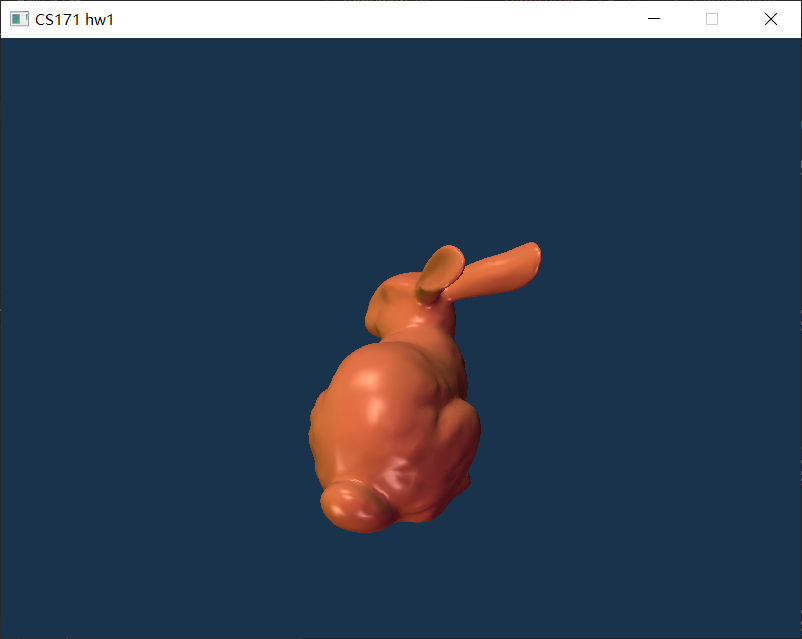
\includegraphics[scale=0.25]{bunny1.png}
		\end{minipage}
		\\
		\begin{minipage}[b]{.4\linewidth}
			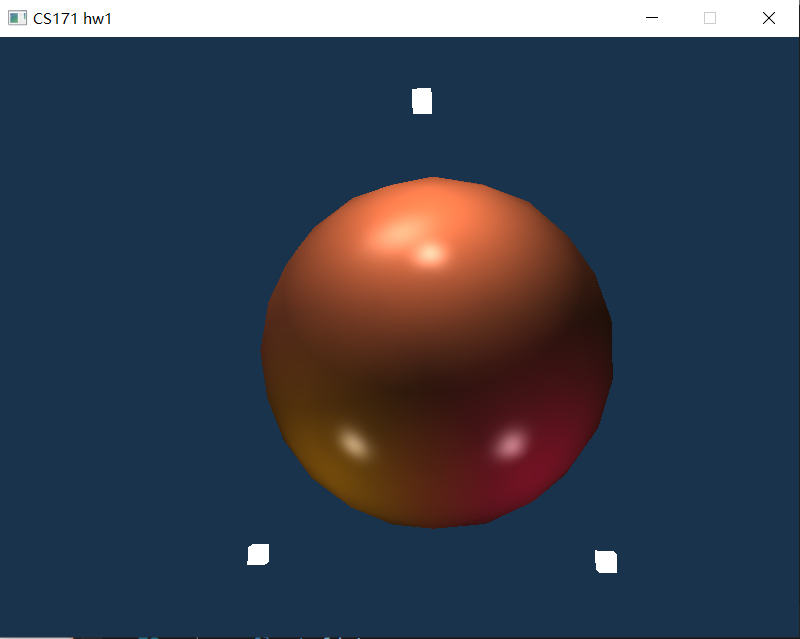
\includegraphics[scale=0.25]{sphere.png}
		\end{minipage}
		\\
		\begin{minipage}[b]{.4\linewidth}
			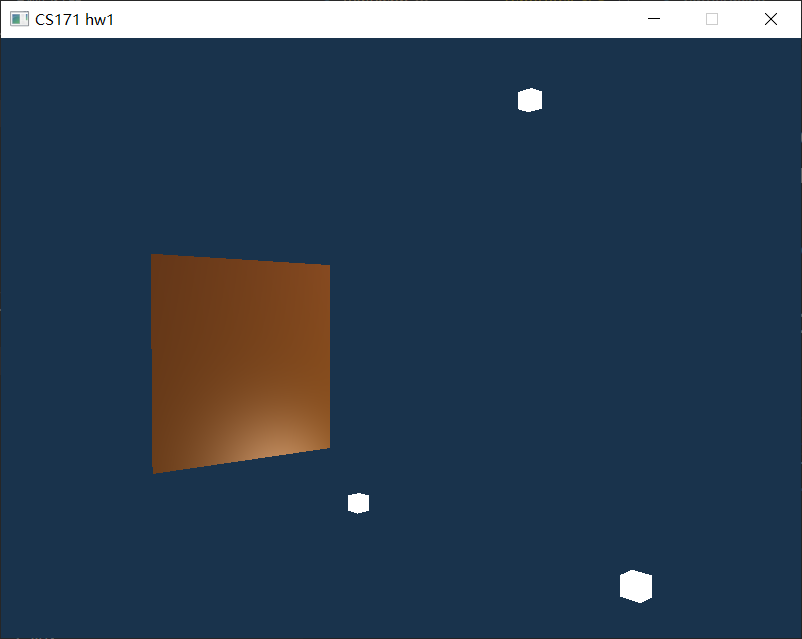
\includegraphics[scale=0.25]{plane.png}
		\end{minipage}
	\end{figure}
\end{document}
